% !TEX encoding = UTF-8 Unicode

\documentclass[a4paper]{article}

\usepackage{color}
\usepackage{url}
\usepackage[T2A]{fontenc} % enable Cyrillic fonts
\usepackage[utf8]{inputenc} % make weird characters work
\usepackage{graphicx}

\usepackage[english,serbian]{babel}
%\usepackage[english,serbianc]{babel} %ukljuciti babel sa ovim opcijama, umesto gornjim, ukoliko se koristi cirilica

\usepackage[unicode]{hyperref}
\hypersetup{colorlinks,citecolor=green,filecolor=green,linkcolor=blue,urlcolor=blue}

%\newtheorem{primer}{Пример}[section] %ćirilični primer
\newtheorem{primer}{Primer}[section]

\begin{document}

\title{Internet marketing\\ \small{Seminarski rad u okviru kursa\\Tehničko i naučno pisanje\\ Matematički fakultet}}

\author{Marina Nešković \\ Anja Petrović \\ Tamara Krstić  \\ Tamara Petrović  \\  }
\date{11.11.2022.}
\maketitle

\abstract{
U ovom tekstu moćićete detaljno da se informišete o internet marketingu. Pročitaćete o istoriji I počecima ovakvog načina reklamiranja, kako se uz pomoć pristupa internetu transformisalo tržište, kao I novonastalim metodama za internet reklamaciju. Ovaj rad pružiće vam informacije o raznim benefitima internet marketinga kao I  odgovor na pitanje zašto je on zapravo koristan.
\tableofcontents

\newpage

\section{Uvod}
\label{sec:uvod}

\\Internet marketing se definiše kao korišcćenje digitalnih kanala za promociju proizvoda ili usluge. Cilj ovog pristupa je povezivanje sa kupcima na mreži – mesto gde provode najviše vremena tražeći informacije ili zabavu. Internet marketing je jako kompleksna grana i složen pojam u koji se može svrstati mnogo toga. Kada krenete da izučavate ovu oblast, onda shvatite da postoji mnoštvo načina na koji se internet marketing sporovodi u praksi. Ako bismo morali da probamo da na najpribližniji i najjednostavniji način objasnimo šta je digitalni marketing, onda bi to bila svaka promocija nekog proizvoda ili usluge putem bilo koje platforme na internetu.
\\ Digitalni marketing je široko u upotrebi, jednostavno zato što postoji toliko mnogo dostupnih kanala za promociju na mreži. Neki od oblika digitalnog marketinga su objavljivanje na društvenim mrežama, email marketing i blogovanje. Bez obzira da li se fokusirate na marketing događaja ili kreirate listu pretplatnika e-pošte, digitalni marketing je neverovatno važan aspekt, jer predstavlja olakšanje današnjem marketingu. Prodavac bilo kada i bilo gde može da stigne do potrošaca: na radnom mestu, kod kuce i sl, kao što i potrošac ima daleko veće mogucnosti za kontaktiranje prodavca.
\\ Prezentovanje na internetu predstavlja reklamu koja ima bitne razlike u svim segmentima reklamiranja u odnosu na standardno reklamiranje.
Internet je stvorio virtualno i globalno tržište oslobođeno granica vremena i prostora. Doprineo je i promeni forme marketinga, od tradicionalnog (masovnog) sa “prosečnim potrošacem” i njemu prilagođenim instrumentima marketinga u marketing miks, u pravcu individualiziranog, prilagođenog (eng. customized), ciljnog (eng. one to one) marketinga. Nova forma marketinga usmerena je na individualiziranog internet potrošaca putem neposredne interakcije. Umesto masovnog marketinga na internetu nastaje marketing mase individua, a oglašavanje se transformiše u izbor informacija.
\\ Marketing se bavi pitanjima i potrebama na tržištu i pronalaskom načina za zadovoljenje tih potreba. Stalno se razvija, zajedno sa razvojem samog tržišta i za cilj ima postavljanje osnove za strategiju poslovanja. Uspeh u marketingu se najčešće dovodi u vezu sa razumevanjem potreba potrošača. U ovakvom konceptu marketing se može definisati kao proces od projektovanja proizvoda i usluga, do cilja, to jest zadovoljenja potrošača.
\\Marketing koncept ima četiri osnovna elementa (poznata kao 4P)\ref{item:uvod} :
\begin{itemize}
    \item Product - proizvod;
    \item Price - cena;
    \item Promotion - promocija;
    \item Placement - distribucija;
    \label{item:uvod}
\end{itemize}
\\ Kombinacija ova četiri elementa se popularno naziva marketing miks.
\\ Nije dovoljno samo napraviti proizvod ili smisliti uslugu. Morate planirati dalji razvoj, morate imati viziju. Svaki proizvod je priča za sebe i čini ga više stvari: karatkeristike, naziv, dizajn, pakovanje, funkcionalnost i tako dalje.
\newpage
\\ Novo područje marketinga sa istom suštinom su pojmovi online marketing, internet marketing, marketing na internetu. Najčešće se definiše kao zadovoljenje potreba i zahteva potrošača za informacijama, proizvodima ili uslugama, uz adekvatnu finansijsku nadoknadu. Pretpostavka uspešne primene online marketinga je znanje o osnovama sistema i procesa marketinga ili često sad već nazvanog tradicionalnog marketinga. To podrazumeva znanja iz područja marketing istraživanja, planiranja i razvoja proizvoda, distribucije i promocije kao aktivnosti marketinga i o instrumentima marketinga.
\\ Dakle, principi i metodi online marketinga potiču od tradicionalnog marketinga a osnovna razlika rezultira u interaktivnosti. Naime, subjekti na strani potrošnje i ponude realizuju dvosmerno komuniciranje. Prodavac bilo kada i bilo gde može da stigne do potrošaca: na radnom mestu, kod kuce i sl, kao što i potrošac ima daleko veće mogucnosti za kontaktiranje prodavca.
\\ Distribucija je mesto gde će se vaš proizvod prodavati. Male prodavnice, veliki marketi, sajt, društvene mreže i tako dalje. Koliko vam je jaka distributivna mreža toliko je jak opseg poslovanja. Potrebno je imati razgranat sistem kroz više nezavisnih kanala. Promocija predstavlja vrstu komunikacije koju marketinški stručnjak može da upotrebi na tržištu u svrhu promovisanja proizvoda. Ovaj element marketing miksa omogućava da proizvod dođe u svest potencijalnih potrošača te da oni budu upoznati sa postojanjem proizvoda, kao i njegovih glavnih osobina i prednosti. Savremeni marketing traži mnogo više od razvijenog proizvoda i privlačne cene. Potrebna je komunikacija sa trenutnim i budućim - potencijalnim kupcima, kao i saradnicima - posrednicima, dobavljačima ali i javnošću u globalu. A šta je marketing ako nije komunikacija? Svaka savremena kompanija upravlja ozbiljnim sistemom marketing komunikacija. Dobri marketing menadžeri nude relevantne informacije i podstiču kupce da izaberu baš njihov proizvod. Svesni su toga da je njihov zadatak da informišu, podsete i ubede potencijalne klijente da je njihov proizvod najbolji izbor.
\\ Po ovakvoj podeli ovaj vodič bi se bavio oglašavanjem, ali kako su mogućnosti interneta i samih društvenih mreža svakim danom sve veće, svi elementi promocije, ali i drugih 4P elemenata su na ovaj ili onaj način u nekom trenutku vezani za ono što se u narodu zove digitalni marketing, a nema konkretnu definiciju. Ako bismo morali da probamo da na najpribližniji i najjednostavniji način objasnimo šta je digitalni marketing, onda bi to bila svaka promocija nekog proizvoda ili usluge putem bilo koje platforme na internetu.
\cite{uvod}
\newpage

\section{Istorijski osvrt}
\label{sec: Istorijski osvrt}
Ako se osvrnemo na rane početke internet marketinga , primetićemo da su prvi koraci u tom smeru napravljeni 1990-ih godina. Prvi vid marketinga koji se pojavio svodio se na jednostavne web stranice koje su u kraćem tekstu pružale informacije o firmi ili proizvodu. Internet reklamiranje je naglo dobilo na popularnosti 1995. što nam govori i činjenica da je 1994. ukupna potrošnja na internetu iznosila svega 0 dolara, dok je 1996. skočila na 301 milion dolara.
Bilo je i nekoliko pokušaja koji nisu zaživeli na tržištu, kao što su na primer iskačući oglasi (engl. pop- up adverts) koji su ubrzlo neutralizovani pomoću određenih programa koji ih blokiraju.
Nagla popularnost društvenih mreža, i društvenog veba pre svega, koja je počela 2006. godine dovela je do nove vrste marketinga koja unosi fundamentalne promene u ono što je do tada bilo smatrano internet marketingom. Uvedena su dva važna koncepta a to su filtrirana pretraga i preporučeni sadržaj za pojedinačnog potrošača.
\subsection{Primeri digitalnog marketinga }
\label{subsec:primeri}
\\ Hotmail je jedan od prvih koji je nudio usluge web pošte i to uspešno. Ova kompanija uspela je da do 1996. stekne 500 hiljada korisnika. Ovaj broj se naknadno još više povećao kasnije kada se njihova ponuda znatno unapredila nudeći korisnicima da se naprave svoj lični besplatni nalog.
\\Još jedan primer uspešnog marketinga jeste Google. Do vremena kada je Google dospeo na tržište 1998. godine, pretraživači interneta su već bili poznati.Google je koristio pametne strategije: odvojio je od sebe sajtove portala pojačavajući fokus na pretragu sa minimalističkim interfejsom koji je sadržao jedva malo više od loga kompanije i trake za pretragu. Preokret i skok popularnosti Google dobija kada uvede novu uslugu (engl. adWords service), koja se svodi na to da trgovci mogu da "licitiraju" za određene ključne reči. Drugim rečima, kada potrošači, korisnici internet pretraživača, ukucaju u svojoj pretrazi određene ključne reči kao rezultati pojavljuju se reklame onih poslodavaca koji su licitirali za te ključne reči.
\\Noviji primer uspešnog internet reklamiranja jeste film naučne fantastike po imenu "Okrug 9"(engl. "District 9"). Film je bio reklamiran lokalno ali i širom sveta isključivo preko interneta. Marketinška strategija im je bila vrlo pametna, koristili su podmetanje zakona o rasnim jednakostima kroz razlikovanje ljudi od vanzemaljaca. Širokim masama se ovaj koncept dopao i stekao je ogromnu popularnost na društvenim mrežama. Međutim, pravi efekat se video tek nakon premijere filma. Masa zadovoljnih gledalaca je svoje utiske delila na internet portalima i time podsticala druge da pogledaju film. Ubrzo, ovaj film je postao jedna od glavnih tema širom sveta i time postao svetski fenomen.
\\\\
Kroz istoriju internet je sam sebe menjao mnogo puta i te promene verovatno nisu ni blizu svog kraja. Međutim, jedna od njegovih danas najvećih primena jeste internet poslovanje. Ljudi danas sve više i više vremena provode na internetu, koristeći online kupovinu, banku, održavajući kontakt sa drugima i ostajući u toku sa dešavanjima. Bez obzira na to kakva je budućnost internet marketinga, neosporno je to da je jedna od većih prekretnica današnjice.\cite{istorija}

\section{Prednosti internet marketinga}
\label{sec:prednosti}
Osnovne prednosti internet marketinga su nepostojanje geografskih barijera, cena efektivnosti, široka publika, personalizacija i dostupnost internet marketinga 24 sata dnevno.
\\Jedna od važnih prednosti je takođe njegovo dejstvo na mala i srednja preduzeća, tako što im povećava broj mogućih kupaca. Zapravo, internet stvara neku vrstu demokratizovanog okruženja gde svi podjednako imaju pravo na reklamiranje i svi imaju relativno iste šanse za uspeh.
\\Internet omogućava brisanje geografskih barijera, kao što smo već rekli, on to čini tako što omogućava neograničen globalni doseg sa izuzetno nižim cenama. Prodavci na internetu sada imaju mnogo veću publiku i mogućnost da svoje proizvode reklamiraju širom sveta svim korisnicima. Imaju mogućnost da se reklamiraju kod svakoga ko ima pristup internetu, što stvara i znatno veću konkerenciju ali i znatno veći broj izbora za potrošače.
\\Putem interneta do željene ciljne grupe se stiže mnogo efektnije.
Jedna od ključnih karakteristika potpunog internet marketinga je da su digitalni marketinški alati su dizajnirani da ciljaju određene grupe kupaca ili publike. Za razliku od tradicionalnih masovnih medija marketing gde se reklame emituju svima. Marketing privlači ciljane kupce koji posebno traže brendove, proizvode ili usluge na koje je fokusirana određena digitalna marketinška kampanja. Takođe, kupci mogu pomoću određenih filtera da svedu svoju pretragu na tačno ono što traže, dok ukoliko nemaju tačno određen predmet internet nudi preporučene pretrage koje su uglavnom personalizovane.
\\Marketinški alati u realnom vremenu mogu doneti preduzećima više koristi od drugih alata. Internet marketing karakterišu interakcije u realnom vremenu koje mogu mnogo više da povežu vaše poslovanje
efikasno sa ciljanim kupcima. Ono što dobijate su trenutni rezultati vaših marketinških napora. Rezultati su natprosečne konverzije za prodaju svaki put kada ciljani kupac posećuje vaše odredišne stranice ili veb-sajtove.
\\U poređenju sa tradicionalnim marketingom u masovnim medijima,internet marketing je mnogo isplativiji. Internet marketing takođe ne zahteva  velika ulaganja kao šta su preduzeća radila u prošlosti sa marketingom u masovnim medijima. Ovakav marketing jeftiniji je u poređenju sa tradicionalnim, a u mnogim slučajevima veb lokacije mogu generisati saobraćaj čak i besplatno. Na slici \ref{fig:prednosti} možemo da vidimo rezultate istraživanja rađenog na ovu temu.
\cite{benefiti i mane}

\begin{center}
    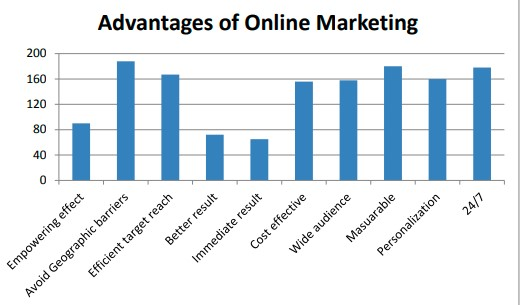
\includegraphics[width=5cm]{13_KrsticPetrovicNeskovicPetrovic/slika.benefiti.marketinga.jpg}\\
    \large{Slika 1: Prednosti internet marketinga}
\end{center}
\label{fig:prednosti}

\\U sledećoj tabeli \ref{tab:tabela1}  se mogu primetiti osnovne razlike izmedju internet i tradicionalnog marketinga. Kroz nju se jasno vide prednosti internet marketinga :
\newpage
\begin{table}[h!]
\begin{center}
\caption{Razlike}
\begin{tabular}{|c|c|c|} \hline
           & tradicionalan marketing& internet marketing\\ \hline
dopire do& ograničenog broja ljudi & globalno\\   \hline
pristupačnost &ograničena&široka i raznolika\\ \hline
komunikacija &jednosmerna&dvosmerna\\\hline
vreme pristupanja&ograničeno&uvek dostupno i veoma brzo\\ \hline
ciljanje dobre  publike&teško&lako\\ \hline
\end{tabular}
\label{tab:tabela1}
\end{center}
\end{table}



\section{Mane internet marketinga}
\label{sec:mane}
Pored mnogih prednosti,internet marketing naravno ima i svoje mane.
\\Ponekad ljudi bolje prihvataju tradicionalan način marketinga nego moderan(preko interneta).Evo i nekih primera zašto:
\\\textbf{Kopiranje}:Internet marketing je osmišljen tako da je dostupan svim korisnicima. Budući da su sve vaše kampanje vidljive, bilo ko može samo da uzme vašu ideju i pretvara se da je njihova.
\\U ovom smislu,dolazi do neoriginalsnoti i ponavljanja već vidjenih kampanja. Vaš projekat nikad neće moći da bude poseban i unikatan.
\\\textbf{Nered na internetu}:
Zbog postojanja internet trolova(eng.trolls), spemera(eng.spammers) i ostalih sumnjivih identiteta i prevaranata na digitalnom tržištu, internet je pun nereda i beskorisnih informacija. Ovo otežava uspeh kompanija da privuku potrošače reklamama preko interneta. Iz ovih razloga, neki potrošači su navikli da ignorišu internet ponude, jer nisu sve zagarantovano korisne.
\\\textbf{Da li odgovara vašem proizvodu?}:
Neki proizvodi prosto ne odgovaraju promociji na internetu. Dobar primer bi bili proizvodi za penzionere, s obzirom da većina penzionera ne koristi internet.
\\\textbf{Konkurencija}:
Kao što je već rečeno u odeljku za kopiranje,internet je svima dostupan, pa samim tim postoji mnogo različitih kampanja koje predstavljaju veliku konkurenciju. Svi se takmiče za najviše pažnje, ali da bi se to izvelo moralo bi da se uloži dosta novca.
\\\textbf{Negativni komentari}:
Negativni komentari i kritike mogu drastično da utiču na uspeh marketinga. Sa razvojem društvenih mreža, sada je dovoljan samo jedan negativan komentar da bi se proširio loš glas o vašem proizvodu.
\\\textbf{Tehnologija je sklona kvaru}:
 Internet zavisi od modernih tehnologija, a one su sklone kvaru i greškama u sistemu .
\\Stvari kao što su linkovi koji ne rade,nefunkcionalni tasteri ili pad sistema, mogu znatno pogoršati vašu kampanju.
\cite{benefiti i mane}
\\Na slici \ref{fig:mane} može se bolje uočiti uticaj ovih problema.
\begin{center}
    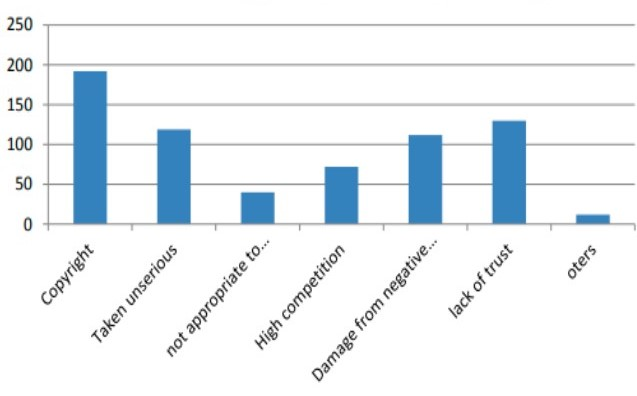
\includegraphics[width=4cm]{13_KrsticPetrovicNeskovicPetrovic/slika.mane.marketinga.jpg}\\
    \large{Slika 2 : Mane marketinga}
\end{center}
\label{fig:mane}
\section{Najvažniji elementi}
\label{sec:najvažniji elementi}
Svaki segment online kampanje samo je deo jednog velikog sistema. Iako je na prvi pogled reč o posebnim segmentima, rezultati su vidljivi samo ako su međusobno dobro sinhronizovani. Naravno, nećete uvek koristiti sve komponente, odluku ćete donositi od slučaja do slučaja. Generalno, što je kompleksniji zadatak, to će biti korišćeno više resursa.
\subsection{Search Engine Optimization(SEO)}
\label{subsec:SEO}
\\\textbf {Search Engine Optimization (SEO)} odnosi se na aktivnosti oko sajta, tako da se on može lako pronaći u internet pretragama. Kada pretražujemo nešto preko interneta, rezultat pretrage će zavisiti od reči koje smo uneli. Zbog toga je jako bitno uneti ključne reči koje što bliže opisuju vaš proizvod. Ovime ćete se bolje pozicionirati na pretragama
\begin{primer}
Bolje se rangira ako su ključne reči -duga svečana haljina  , nego samo -haljina.
\end{primer}
\subsection{Email marketing}
\label{subsec:Email}
\\\textbf{Email marketing} je i dalje izuzetno efikasan način da se kontaktira sa klijentima. Ukratko, reč je, pre svega, o promotivnim emailovima kojima je osnovni cilj da se ostvari uspešan kontakt i prenesu marketinške poruke.
\\Na ovaj način se obraćamo potencijalnim kupcima, ali i starim korisnicima usluga koje želimo da upoznamo sa novim poslovnim prilikama.
\\Tipične vrste mailova su prikazane na ovoj listi \ref{item:email}:
\begin{itemize}
    \item Poziv na pretplatu na newsletter;
    \item Promocije;
    \item Briga o kupcima (popust za rođendan, specijalne promocije u okviru loyalty programa…);
    \item Email zahvalnica nakon kupovine;
    \label{item:email}
\end{itemize}
\\Zbog zloupotrebe ovog vida promocije , email klijenti  Gmail i Hotmail su razvili filere koji  blokiraju beskorisne ili prevarantske emailove (spam).
\subsection{Pay per Click (PPC)}
\label{subsec:PPC}
\\\textbf{Pay Per Click (PPC)} se odnosi na digitalno oglašavanje koje se plaća po kliku, tj. akciji korisnika. To može da bude kliktanje na sponzorisani post, link ili baner(eng.banner) koji ste platili.
\\To praktično znači da možete da kupite posete vašem sajtu ili lajkove na društvenim mrežama kao što su Facebook, Instagram ili Twitter. Za ove aktivnosti najčešće se koriste Google Ads ili Facebook Ads alati.
Prednost PPC kampanja je to što mogu da donesu trenutne rezultate usled preciznog ciljanja publike.Ovime možete da izaberete ko će videti vaš oglas na osnovu pola, starosti, lokacije, zanimanja, jezika...
\\Ovaj vid kampanje je dosta efikasan ,al može da bude i jako skup.
\subsection{Social Media Marketing}
\label{subsec:Social Media}
\\\textbf{Social media marketing} koristi društvene mreže kako bi promovisao brend i komunicirao sa potrošačima. Promotivne aktivnosti na društvenim mrežama fokusiraju se na najpopularnije platforme kao što su Facebook, Instagram, Linkedin, Twitter, Snapchat, Pinterest i druge. Svaka društvena mreža ima drugačiju publiku, pa se i promotivne aktivnosti razlikuju.
\\Samim tim, brend se najviše približava korisnicima, predstavljajući razne ideje kroz razne oblike aktivacije. U tu svrhu se često koriste i poznate ličnosti koje utiču na stavove svojih fanova. Oni na ovaj način utiču na javno mnjenje, pa se zbog toga ove poznate osobe zovu i – influenseri.
\subsection{Affiliate marketing}
\label{subsec:affiliate marketing}
Zamislite da posećujete stranicu na kojoj se nalazi lista najboljih filmova 2022 godine, isečci najboljih scena u tim filmovima njihova kritika i njihovi glumci. Vi ste došli na tu stranicu da bi ste videli kritiku nekog od tih filmova ali sada vam se bas gleda taj film! Srećom  na tom sajtu se nalazi link preko koga mozete da kupite članstvo platforme na kojoj možete da ga pogledate. 

Taj sajt je upravo uspešno reklamirao tu platformu za gledanje filmova uz pomoć linka koji void na tu platformu. \textbf{Afiliate marketing} je tip marketinga koji koristi popularnost nekog sajta da reklamira neki proizvod ili uslugu koja je blisko povezana sa sa temom tog sajta. 
Ovakav način marketinga trazi saradnju vlasnika sajta I prodavca uz pomoć koje vlasnik sajta za za svaku prodaju ili definisanu radnju posetilaca sajta dobiti neku proviziju a prodavac dobija željenu reklamu.







\subsection{Search Engine Marketing(SAM)  }
\label{subsec:SAM}
Strategija \textbf{Search Engine Marketinga(SAM)} jeste korišćenje SEO I PPC metoda kako bi se osihgurala što bolja pozicija tokom pretraživanja. To se nekada izvodi korišćenjem ključnih reči da bi se sto bolje objasnio dati proizvod ili ulaganjem u pay per click (eng plaćanje po kliku). Osiguravajući bolje mesto tokom pretrage povećava se broj kupaca koji će videti proizvod, a samim tim I kupiti ga.

 U zavisnosti od platforme preko koje se sprovodi reklamacija pretraživač ce raditi drugačije i to se uvek mora uzeti u obzir radi maksimalne efikasnosti. Da li ce to biti stavljanje dovoljnog broja heštegova sa ključnim rečima na društvenim mrežama (na slici \ref{fig:instagram}
 prikazan je primer hestagova na instagramu) na određen sadržaj ili tačni I jasni nazivi zavisi na sta se pretraživač te platforme najviše fokusira.


\begin{center}
    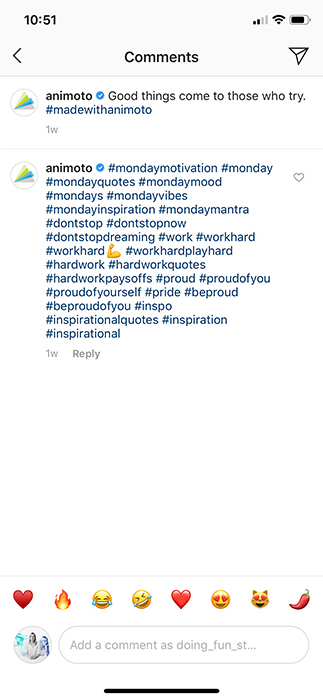
\includegraphics[width=5cm]{13_KrsticPetrovicNeskovicPetrovic/instagramh.jpg}\\
    \large{Slika 3:hestagovi na instagram postu}
\end{center}
\label{fig:instagram}

\subsection{Content Marketing  }
\label{subsec:Content}
Content marketing je oblik marketinga koji koji se krije iza sadrzaja neke stranice. Ovaj oblik reklamacije stavlja određeni proizvod unutar sardržaja kao nesto pomoću čega se dati sadržaj odvija I reklamira ga kao nezaobilazan deo radnje tog sadržaja. 

Za ovaj način marketinga koriste se platforme koje za cilj imaju proizvodnju zanimljivog sadrzaja kao što su društvene mreze I blogovi. Ovakvi sadržaji ce privlačiti potrošače kojima su ovakve teme bliske I zanimljive, pa će tako biti I zainteresovani za reklamirani proizvod. 

Na  primer zamislite da prodajete pribor za slikanje. Umesto da samo postavite kako prodajete pribor, možete napraviti blog na kome će te objašnjavati tehnike slikanja I postavljati slike koje su baš rađene priborom koji vi prodajete!
\cite{elementi}
\cite{hollistic}

\section{Zaključak}
\label{sec:zakljucak}
Iako na starije generacije više utiču druge vrste reklamiranja kao što su reklame na bilbordima ili preko TV-a, budućnost marketingase svodi na reklamiranje preko društvenih mreža I veb stranica na internetu postaje sve uticajnije dok ostali oblici reklamiranja postaju manje rasprostranjeni. Danas, reklamiranje nekog proizvoda mnogo uspešnije se može obaviti preko interneta jer nekada ograničeno tržište se proširuje na ceo svet I tako stiče velika prednost u odnosu na ostale načine reklamacije I zato predstavlja veoma dobar način reklamiranja danas.

Iako razne stranice na internetu dobijaju značajan profit od raznih oblika reklama, one moraju da budu umerene u količini reklama jer prevelikom količinom reklama mogu da dosade korisniku sajta I da se tako smanji njegova posećenost a tako I korist tih reklama. Dobri oblici internet marketinga imaju za svoj zadatak ka suptilno  upute korisnika ka svojim proizvodima. Mnoge firme različitih zanimanja vide korist I značaj internet marketinga I ulažu dosta vremena I novca u njega kako bi proširile svoj posao I povećale broj potrošača. 

Iako se internet marketing menja I konstantno proširuje jedan je od veoma važnih grana marketinga I konstantno doprinosi uspehu velikog broja firmi I biznisa svojom dostupnošću I rasprostranjenošću I kao takav je jedan od najbitnijih oblika marketinga danas.
\addcontentsline{toc}{section}{Literatura}
\appendix

\iffalse
\bibliography{seminarski}
\bibliographystyle{plain}
\fi

\begin{thebibliography}{9}
\bibitem{uvod} mailchimp.com,https://mailchimp.com/marketing-glossary/digital-marketing, 12.11.2022. 
\bibitem{istorija} Alex Trengove. \emph{Internet marketing}. 2021.

\bibitem{benefiti i mane} Yurovskiy, Vladislav \emph{Pros and cons of internet marketing} 2014.
\bibitem{elementi} IT-akademija.com,https://www.it-akademija.com/digitalni-marketing-kompletan-vodic,12.11.2022.
\bibitem{hollistic} Holisticdigitalsolutions,https://holistic-digital.com/internet-marketing/,14.11.2022.



\end{thebibliography}


\appendix



\end{document}
